% compile with: lualatex -shell-escape filename.tex
\documentclass[tikz]{standalone}
\directlua{luatexbase.add_to_callback(
  "wrapup_run",
  function() os.execute("pdf2svg \jobname.pdf \jobname.svg") print("Converted to SVG.") end,
  "final callback to convert pdf file")}

\usetikzlibrary{matrix}

\newcommand\FenwickTree[2]{ % anchor, data rows
  \matrix[
  at=(#1),
  anchor=north,
  draw,
  matrix of nodes,
  ampersand replacement=\&,
  column sep=3pt,
  nodes={minimum height=2em, text width=1cm, align=center, anchor=base},
  ]{
    \node{pos}; \& \node{AIB}; \\
    \node{...}; \& \node{...}; \\
    #2
    \node{...}; \& \node{...}; \\
  };
}

\begin{document}

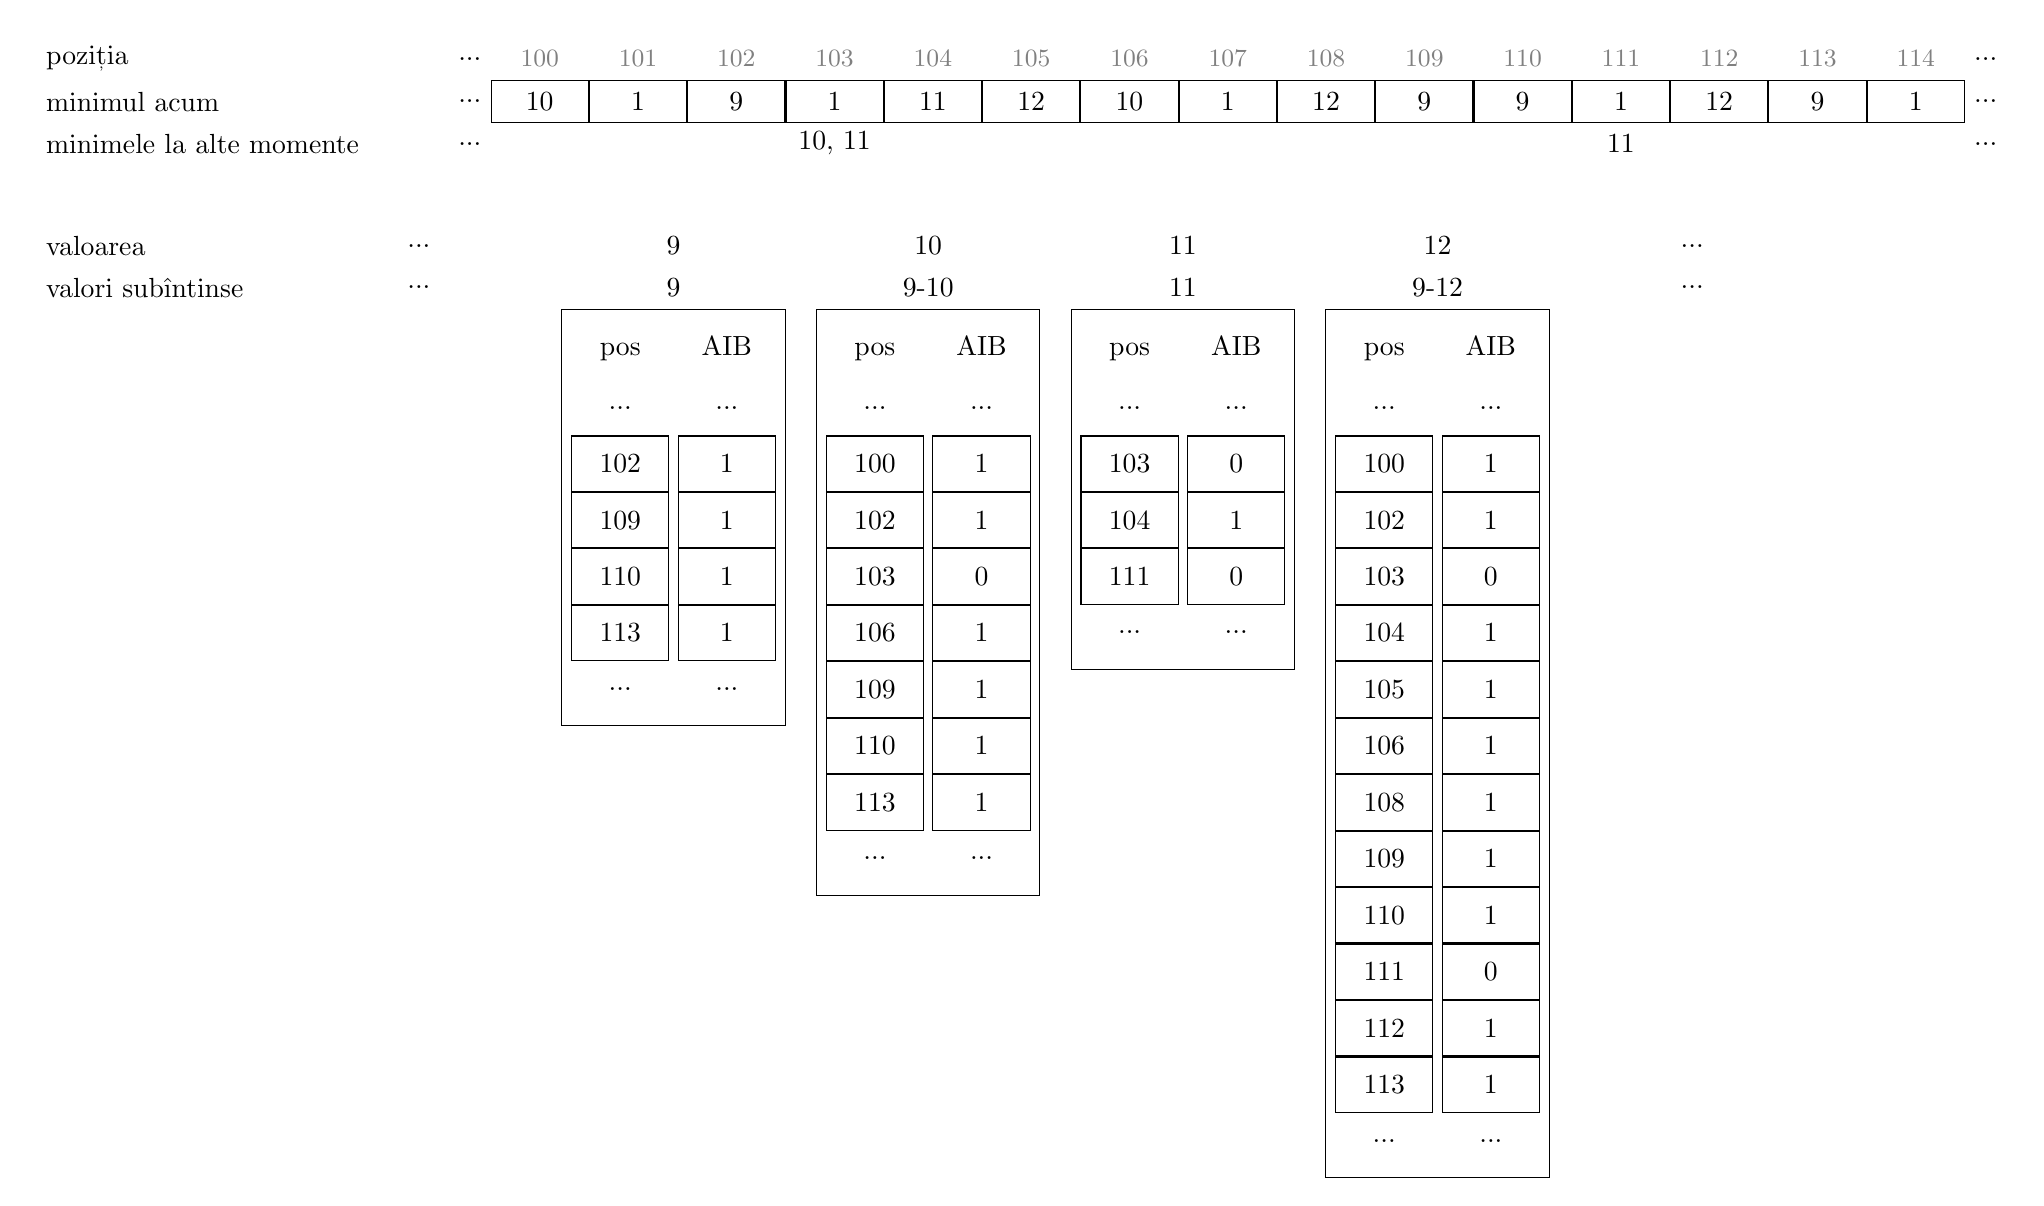
\begin{tikzpicture}[]
  % Contents of a slice of the array of minima.
  \matrix[
  anchor=west,
  align=left,
  nodes={minimum height=1.5em, align=center, anchor=center},
  header/.style={text width=5cm, align=left},
  vpos/.style={text width=1cm, font=\small, text=black!50},
  val/.style={draw, text width=1cm},
  ]{
    \node[header]{poziția}; & \node{...}; & \node[vpos]{100}; & \node[vpos]{101}; &
    \node[vpos]{102}; & \node[vpos]{103}; & \node[vpos]{104}; & \node[vpos]{105}; &
    \node[vpos]{106}; & \node[vpos]{107}; & \node[vpos]{108}; & \node[vpos]{109}; &
    \node[vpos]{110}; & \node[vpos]{111}; & \node[vpos]{112}; & \node[vpos]{113}; &
    \node[vpos]{114}; & \node{...}; \\

    \node[header]{minimul acum}; & \node{...}; & \node[val]{10}; & \node[val]{1}; &
    \node[val]{9}; & \node[val]{1}; & \node[val]{11}; & \node[val]{12}; &
    \node[val]{10}; & \node[val]{1}; & \node[val]{12}; & \node[val]{9}; &
    \node[val]{9}; & \node[val]{1}; & \node[val]{12}; & \node[val]{9}; &
    \node[val]{1}; & \node{...}; \\

    \node[header]{minimele la alte momente}; & \node{...}; & & & & \node{10, 11}; &
    & & & & & & & \node{11}; & & & & \node{...}; \\
  };

  % Contents of the Fenwick tree of columns (values).
  \matrix[
  anchor=west,
  align=left,
  yshift=-6em,
  nodes={minimum height=1.5em, text width=3cm, align=center, anchor=center},
  header/.style={text width=3cm, align=left},
  ] {
    \node[header]{valoarea}; & \node{...}; & \node{9}; & \node{10}; & \node{11}; &
    \node{12}; & \node{...}; \\

    \node[header]{valori subîntinse}; &
    \node{...}; &
    \node (val-9) {9}; &
    \node (val-9-10) {9-10}; &
    \node (val-11) {11}; &
    \node (val-9-12) {9-12}; &
    \node{...}; \\
  };

  % Fenwick tree for value 9.
  \FenwickTree{val-9.south}{
    \node[draw]{102}; \& \node[draw]{1}; \\
    \node[draw]{109}; \& \node[draw]{1}; \\
    \node[draw]{110}; \& \node[draw]{1}; \\
    \node[draw]{113}; \& \node[draw]{1}; \\
  }

  % Fenwick tree for values 9-10.
  \FenwickTree{val-9-10.south}{
    \node[draw]{100}; \& \node[draw]{1}; \\
    \node[draw]{102}; \& \node[draw]{1}; \\
    \node[draw]{103}; \& \node[draw]{0}; \\
    \node[draw]{106}; \& \node[draw]{1}; \\
    \node[draw]{109}; \& \node[draw]{1}; \\
    \node[draw]{110}; \& \node[draw]{1}; \\
    \node[draw]{113}; \& \node[draw]{1}; \\
  }

  % Fenwick tree for values 11.
  \FenwickTree{val-11.south}{
    \node[draw]{103}; \& \node[draw]{0}; \\
    \node[draw]{104}; \& \node[draw]{1}; \\
    \node[draw]{111}; \& \node[draw]{0}; \\
  }

  % Fenwick tree for values 9-12.
  \FenwickTree{val-9-12.south}{
    \node[draw]{100}; \& \node[draw]{1}; \\
    \node[draw]{102}; \& \node[draw]{1}; \\
    \node[draw]{103}; \& \node[draw]{0}; \\
    \node[draw]{104}; \& \node[draw]{1}; \\
    \node[draw]{105}; \& \node[draw]{1}; \\
    \node[draw]{106}; \& \node[draw]{1}; \\
    \node[draw]{108}; \& \node[draw]{1}; \\
    \node[draw]{109}; \& \node[draw]{1}; \\
    \node[draw]{110}; \& \node[draw]{1}; \\
    \node[draw]{111}; \& \node[draw]{0}; \\
    \node[draw]{112}; \& \node[draw]{1}; \\
    \node[draw]{113}; \& \node[draw]{1}; \\
  }
\end{tikzpicture}

\end{document}
